\chapter{Inductive learning}
\label{ch:machine-learning}
\begin{flushright}
\emph{Rewards and punishment is the lowest form of education.}\\
--- Zhuangzi (4th Century BC)
\end{flushright}
\minitoc

Note:  reinforcement learning is discussed in \S\ref{sec:RL}.

\section{``Learn by being told''}
\label{sec:learn-by-being-told}

This is probably the most efficient learning method.  (As Martin Magnusson pointed to me, \citep*{Perlis1996} explored the possibility where a human is able to teach an AI via natural-language conversations.  The paper contains hypothetical examples of some such conversations.)

\textbf{The Tell-Learn loop.}  Translate a natural language sentence into a logical formula.  Then the logical formula will directly enter the KB as knowledge, which is a very efficient way of learning.

The main difficulties in this loop are:
\begin{compactenum}[1.]
\item  The assimilation of the fact into the KB, which requires belief revision
\item  The translation from natural language to logic;  sometimes this require abductive reasoning even when the NL parser does an adequate job
\item  Surprisingly, inductive learning is also needed (see below)\\
\end{compactenum}

The base logic should be:\\
1. simple, for machine learning\\
2. close to NL, for easy translation from NL to logic.

\section{What is inductive logic programming?}
\label{sec:inductive-learner}

Inductive learning using logic is studied under the heading ILP (inductive logic programming; an excellent and up-to-date survey of which is \citep*{Konstantopoulos2008}).  The area known as theory revision is also essential to AGI (an excellent new book on ILP that discusses theory revision is \citep*{DeRaedt2008}).  Other notable books on induction / ILP are: \citep*{Holland1986}, \citep*{Muggleton1992}, \citep*{Lavrac1994}, \citep*{Bergadano1996}, \citep*{Nienhuys-Cheng1997}, \citep*{Flach2000}, \citep*{Lloyd2003}, \citep*{Getoor2007}, \citep*{DeRaedt2008}.

Induction is the dual of abduction:  both seeks a hypothesis $H$ to explain an example $e$:\\
\hspace*{1cm} $H \cup KB \vdash e$\\
\hspace*{1cm} abduction seeks an $H$ that is a ground fact\\
\hspace*{1cm} induction seeks an $H$ that is a general rule (ie, containing variables)

\textbf{Why is ILP needed?}  From my observations, when people use natural language to express ideas, they usually leave many \textbf{gaps} that must be filled by abductive or inductive reasoning.  A parser can translate NL sentences into logic \textit{literally}, but the resulting KB would be incapable of reasoning.

Filling in the logical gaps is very hard for humans because the inference of the gaps are inaccessible to conscious thinking.  Therefore, an inductive machine learner is required to perform this function.

\section{Examples}

\textbf{A. ``Women usually have long hair''}

Example facts:\\
\hspace*{1cm} Mary is a girl, Mary has long hair\\
\hspace*{1cm} Jane is a girl, Jane has long hair\\
\hspace*{1cm} John is a guy, John has short hair\\
\hspace*{1cm} etc...\\
To learn:\\
\hspace*{1cm} female(X) $\rightarrow$ long-hair(X)\\

This example illustrates the \textbf{MDL principle}:  The general rule \textit{covers} many examples and thus is \textit{compressive} -- In some situations, we may forget individually which woman has long hair, while remembering a group of women as mostly having long hair (eg, after seeing a group of choir singers).

We can make this example more complex by adding the role of a speaker:\\
\hspace*{1cm} The teacher tells me ``Mary has long hair''\\
\hspace*{1cm} The teacher tells me ``Mary is a girl''\\
\hspace*{1cm} The teacher tells me ``Jane has long hair''\\
\hspace*{1cm} The teacher tells me ``Jane is a girl''\\
\hspace*{1cm} etc...

We can have the general rule:
\footnote{In this example we have used 3 tricks:\\
a. propositions as variables\\
b. quoted formulae\\
c. equality\\
just for the sake of illustration.  The actual KR scheme is still undecided.}\\
\hspace*{1cm} \textit{``If a speaker is a credible source, then what s/he says can be assumed to be true''}\\
\hspace*{1cm} \textbf{R1:} \quad credible(X) $\wedge$ says(X,Y) $\rightarrow$ Y

But notice that R1 can cover the girls examples only if we include the quoted sentences:\\
\hspace*{1cm} \begin{tabular}{l l}
R1 $\wedge$ Y=long-hair(mary) & $\vdash$ long-hair(mary)\\
R1 $\wedge$ Y=female(mary)    & $\vdash$ female(mary)\\
R1 $\wedge$ Y=long-hair(jane) & $\vdash$ long-hair(jane)\\
R1 $\wedge$ Y=female(jane)    & $\vdash$ female(jane)
\end{tabular}

Thus, we can further compress the right hand sides with this rule:\\
\hspace*{1cm} \textbf{R2:} \quad female(X) $\rightarrow$ long-hair(X)\\
or compress what the teacher says:\\
\hspace*{1cm} says(teacher,"female(X) $\rightarrow$ long-hair(X)")

This shows that even when an example is explained (entailed) by a general rule (R1), it may still require compression (R2).  This is different from the traditional ILP goal which is simply to ``cover'' (ie entail) positive examples.  Now we need to find \textit{all possible} ways to compress the KB.

\textbf{B. Roman numerals}

Example facts:\\
\hspace*{1cm} Roman numeral 1 is \code{I}\\
\hspace*{1cm} Roman numeral 2 is \code{II}\\
\hspace*{1cm} Roman numeral 3 is \code{III}\\
To learn:\\
\hspace*{1cm} Roman numeral $n$ is $n$ \code{I}\\
(which is wrong, but is reasonable in common sense).

\section{Structure of the hypothesis space}
\label{sec:subsumption-peaking}

A very important concept is that the logical hypothesis space is structured by the \textbf{subsumption order}:
\begin{figure}[H]
\centering
\includegraphics[scale=1]{rules-tree.png}
\end{figure}

An interesting phenomenon is that the probabilistic truth value of a branch of hypotheses follows a peaking pattern as we move along the specialization direction:
\begin{figure}[H]
\centering
\includegraphics[scale=1]{subsumption-peaking.png}
\end{figure}
Actually the truth value can stay constant along a branch that specializes by adding synonymous conjuncts until such synonyms run out.  Also, the truth value may actually \underline{decrease} when a conjunct is added and then increase again when other conjuncts are added.  For example, a non-obvious idea that spreads virally will make a startup successful, but each conjunct alone may decrease the truth value.  So the search of rules cannot be pruned prematurely.

But that is the situation of rules search.  During deduction our concern is of rule satisfaction.  During deduction there is no need to try rules that are past the maximum, they may constitute the \textbf{frontier} of rules search.

\section{Complexity}

\subsection{Inducing one hypothesis}

The main task of ILP is to search in the hypothesis space $\Hyp$ specified partly by the logical syntax (such as $\catPZ$ logic) and partly by background knowledge (eg what kind of predicates are present).  The hypothesis space is structured into a lattice with a partial order (usually denoted $ \preceq $).  The partial order can be one of \textbf{$\theta$-subsumption}, LGG (\textbf{least general generalization}), or \textbf{logical entailment}.  These have subtle differences, with logical entailment being the most rigorous.  The searcher can traverse up and down the lattice, corresponding to \textbf{generalization} and \textbf{specialization} of the hypothesis.  These 2 are known as \textbf{refinement operators}.  Because there are so many ways to generate hypotheses in FOL (with many predicates to choose from, and the possibility of introducing variables as desired), the branching factor is extraordinarily high.  Also, the lattice can be infinite, so we need to limit its depth.

Another problem is that, once a hypothesis has been generated, it must be tested against the rest of the KB for \textbf{consistency}.  The consistency check must also be limited in depth, but even then it is very time-consuming.

Much of the complexity of induction occurs in the ``inventive step'', whereby a new rule is generated.  The inventive step can draw upon knowledge from the entire KB, which makes it combinatorially explosive.  Currently the most promising idea I have is to ``recall similar examples'' -- that means, we perform an \textbf{associative memory search} to recall examples similar to the current experience, and only then do we try to generalize from the experience plus the recalled examples.  But this strategy merely pushed the responsibility to the associative memory to recall only the most \textbf{salient / relevant / interesting} examples.  Still, this trick seems to be more efficient than blind search.

Another promising idea is that some of the more intensive processing can be performed during \textbf{sleep}.

\subsection{Inducing a whole theory}
\label{sec:complexity-of-hypothesis-space}

Let $\Hyp$  denote the hypothesis space (ie, space of all logic formulae).  The size of $\Hyp$ is huge (see above).\\
A logical theory $T$ is a set of hypotheses, $ \{ h_i | h_i \in \Hyp \} $.  Note that $ T \in 2^{\Hyp} \;$ which is a hugely huge space.\\
Let $E$ denote the set of examples $\{ e_1, ... \}$ that should be covered by the target theory.\\
So we're seeking an optimal theory $T^*$ such that it covers all examples and is succinct, ie:\\
\hspace*{1cm} $ T^* \vdash \{ e_i \} $ \quad and \quad $ |T^*| $ is minimal.

There is hope, since we can \textit{seed} the initial theory with human knowledge.  In other words, we can start with a $T_0$ which contains a large number of logic statements translated from NL.

Even if we do that, we can realistically only store one theory in memory.  When we evaluate a new hypothesis $h$ to cover an example $e$, ie, to test whether\\
\hspace*{1cm} $h \cup T \vdash e \; ?$\\
we have to bear in mind that we are just testing the hypothesis $h$ w.r.t. \textit{one} background theory.  This means that $h$ may have a different score when $T$ changes;  but unfortunately we cannot realistically keep track of different scores of $h$ against different theories.  In other words, the scores we keep will be somewhat \textit{inaccurate} and are \textit{relative} to a constantly changing candidate theory.  \{ TO-DO:  Due to the use of probabilistic logic, we can store multiple sets of hypotheses simultaneously.  Revise this paragraph. \}

\section{Compression}
\label{sec:compression}

In general, compression is achieved via \textbf{pattern recognition} (\S\ref{ch:pattern-recognition}).  Upon the arrival of new sensory input, the Pattern Recognizer is invoked to recognize patterns in the data (the process is forward-chaining).  Due to the use of \textbf{fuzzy} pattern recognition, the result may be lossy, which is good.

\textbf{Decompression} is a special form of abduction:  starting from the recognized patterns (facts) we try to abduce the original low-level sensory facts.  (Though we're usually not interested in low-level facts during normal abduction.)

Inductive learning is a kind of dual of pattern recognition:  whereas pattern recognition recognizes patterns using some logic rules, inductive learning learns those rules.  The job of the Inductive Learner is to generalize from regularities in the sensory input whenever possible, adding new rules to the KB.

In summary:\\
\hspace*{1cm} compression = pattern recognition = forward chaining\\
\hspace*{1cm} decompression = abduction = backward chaining\\
\hspace*{1cm} learning to compress = backward chaining with rule invention

\textbf{Formal definition.}  The goal is to find a theory $T$ to compress a set of examples $E = \{ e_i \}$ such that:\\
\begin{equation}
\left
\{
\begin{array}{c@{\quad\quad}l}
T \vdash \hat{E}  & \mbox{(reconstruction of memory)}\\
\hat{E} \approx E & \mbox{(approximation)}\\
|T| \leq |E|      & \mbox{(smaller description length)}
\end{array}
\right.
\end{equation}
Note:  the entailment $\vdash$ should be fuzzy/probabilistic.

\textbf{About coverage.}  Usually, an example can be covered (entailed) by a number of alternative proofs.  This is probably very common.  For example:\\
\hspace*{0.8cm} \begin{tabular}{l l}
Mary doesn't love John & $\vdash$ John is unhappy\\
John doesn't love Kate & $\vdash$ Kate is unhappy\\
Pete has no money      & $\vdash$ Pete is unhappy
\end{tabular} \vspace{-0.2cm}

but we can further compress the right hand sides by:\\
\hspace*{1cm} everyone is unhappy\\
even though the right hand sides were entailed by 3 different reasons.

Having a large number of general rules enables better \textbf{reconstruction} of past memories.  Better reconstruction is clearly an advantage from a utilitarian perspective as we often do not know in advance what memories may be useful later.  (Overlapping coverage may be a by-product of having a large number of rules.)

We can define \textbf{information utility} as the utility of information items ($U: \{ \mbox{infon} \} \rightarrow \setR$)
\footnote{An infon is informally defined as a discrete information item.  In practice it can be any proposition in the KB.}
, as a generalization of utility over states ($U: \{ \mbox{state} \} \rightarrow \setR$).  Then the goal of compression is to \textit{minimize reconstruction errors (weighted by information utility) with the smallest theory}.  This is in keeping with the MDL principle.

%Note:  $T$ may contain ground facts that are absent in $E$.  For example, we may remember that many women in the choir have long hair (a ground fact in $T$) but we may not remember exactly who has long hair (ground facts in $E$).

%The error $D = \mbox{Diff} (\hat{E}, E)$ is in general very difficult to calculate, as it involves the differences between things like:\\
%\hspace*{1cm} blonde $\approx$ brunette\\
%\hspace*{1cm} chair $\approx$ desk\\
%\hspace*{1cm} humorous $\approx$ witty\\
%which seems to involve a similarity measure (\S\ref{sec:similarity}).  But we can focus on the subclass of \textbf{compressive approximations} where Diff() can be defined more easily.

In traditional ILP with binary logic, we settle at finding a theory that covers all positive examples and none of the negative examples.  In the compression setting, mere coverage is not enough:  we should generate new rules even when the data are already entailed by some existing rules, because the new rules can further compress data.

%A possible scoring function is:\\
%\hspace*{1cm} $S = -kD - |T|$\\
%where $k$ is some constant.
%
%A brute-force algorithm is to search all possible sets of hypotheses ($2^{\mathbb{H}}$) and output the one with the best score, which is obviously impractical.  A local search algorithm may start with a seed theory and try to search in its neighborhood.  For this purpose we need an \textit{incremental} scoring function:\\
%\hspace*{1cm} $\Delta S = -k \Delta D - \Delta |T|$
%
%\begin{algorithm}[H]
%\caption{Naive compressor}
%\alginout{examples $E$}
%{a theory $T$}
%\begin{algtab}
%\alglabel{alg:naive-compressor}
%
%start with a seed theory\\
%
%\algrepeatforever
%	get examples from sensory experience\\
%
%	(randomly/heuristically) add/subtract/modify facts/hypotheses in $T$\\
%
%	if $\Delta S > 0$ accept the changes\\
%\algend
%
%\end{algtab}
%\end{algorithm}
%\vspace{-0.7cm}
%
%The calculation of $\Delta S$ may be time consuming as it involves reconstructing $\Delta\hat{E}$ and then finding the error $\Delta D$.

\subsection{Plateau phenomenon (local minima)}

Some changes in $T$ may increase the error first but further changes in that direction may result in a smaller error.  This phenomenon (ie, local minima) is common in ILP and makes learning more difficult.

An example is given in \citep*{Bergadano1996}, p89, for the learning of the Prolog function \code{append/3}.  The positive and negative examples are:\\
\hspace*{1cm} \begin{tabular}{l l}
$e^+$: & \code{append([0],[1,2],[0,1,2])}\\
       & \code{append([],[1,2],[1,2])}\\
$e^-$: & \code{append([0],[1,2],[0,1])}\\
       & \code{append([0],[1,2],[1,2])}\\
       & \code{append(0,1,[0,1])}\\
       & \code{append(a,b,[a,b])}
\end{tabular}

And the target clause is:\\
\hspace*{1cm} \code{append(X,Y,Z) :- list(X), head(X,X1), tail(X,X2), append(X2,Y,W), cons(X1,W,Z)}

The learning of the first literal, \code{list(X)}, would indeed have positive information gain
\footnote{The definition of information gain is that used by the ILP program FOIL.  See the book for details.}
 as it excludes the last 2 negative examples;  but the addition of the following 3 literals would have small or even negative information gain, until the last literal is reached and all positive and negative examples are covered.

\subsection{Minimum description length}

An interesting observation (noted in \citep*{MacKay2003} Chapter 28, and \citep*{Chater2005}) is the equivalence of MDL and Bayesian likelihood maximization:  Given the data $D$, The goal of perception is to choose the hypothesis $H^*$ that maximizes $P(H|D)$.  According to Bayes theorem, this is equivalent to choosing the $H^*$ that maximizes $P(D|H)P(H)$, where $P(H)$ represents some sort of subjective prior bias.  The $H^*$ that maximizes $P(D|H)$ is the same $H^*$ that minimizes the negative of the logarithm of this term, which can be written:\\
\hspace*{1cm} $-\log_2 P(H) - \log_2 P(D|H)$.\\
By Shannon's coding theorem, the optimal code length for a probability $p$ is $-\log_2 p$, so we can interpret the above as:\\
\hspace*{1cm} codelength($H$) + codelength($D|H$).

Note:  the MDL terminology is different from the logic terminology:\\
\hspace*{1cm} \begin{tabular}{l l l}
\textbf{in MDL}       & \textbf{in logic}\\
\hline
a hypothesis          & is called a logical theory\\
N/A                   & a hypothesis (= part of a logical theory)
\end{tabular}

\{ TO-DO:  How does this shed light on the logical compression algorithm? \}

%\section{Evolutionary algorithms}
%
%It seems that EA, as a global optimization technique, can be a good choice for the ILP search.  There are two general approaches to GA (\citep*{Freitas2002}):
%
%In the \textbf{Pittsburgh approach}, each individual in the EA population represents \textit{a set of rules}, ie, an entire candidate solution.
%
%In the \textbf{Michigan approach}, which departs from conventional EA's, each individual represents \textit{a single rule}, ie, a part of a candidate solution.
%
%It seems to me that we need the Michigan approach.
%
%TO-DO:  how to learn hybrid logical rules.
%Learning of Z rules is based on examples with explicit Z values;\\
%Learning of P rules is based on examples that are true or false.\\
%So they may be learned independently?
%
%Besides Michigan vs Pittsburgh, one more thing is the role of a lot of background knowledge.  How might this change things?

\section{Algorithm}

(Cf algo~\ref{alg:top-level-sensory-processing} for the top-level algorithm of the logical reasoner.)

The goal of the learning algorithm is to produce useful generalizations, or we can say the most \textit{compressive} generalizations.

\underconst
\hrule

\begin{algorithm}[H]
\caption{Practical inductive learner}
\alginout{incoming facts}
{1 or more hypotheses}
\begin{algtab}
\alglabel{alg:practical-inductive-learner}

Try to recall similar examples from memory.\\

Invent a hypothesis to generalize the new fact + examples\\

\end{algtab}
\end{algorithm}
\vspace{-0.7cm}

I look at the problem from a perspective that is slightly different from the one prevalent in the ILP literature.  Most ILP methods search in the \textit{hypothesis space}, but I find it easier to think about the problem in \textit{proof space}:\\

\begin{compactenum}[\textbullet ]
\item  My algorithm searches for explanations of \textit{one incoming fact} while inventing (possibly many) hypotheses along the way.

\item  The hypothesis-space algorithm, on the other hand, focuses on \textit{one hypothesis}.  It would pick some examples (past or incoming facts) and move around the hypothesis lattice in order to cover them, ie, keeping a score of the numbers of positive and negative examples that are covered or not.  And it seeks the hypothesis with the best score.\\
\end{compactenum}

%A problem with hypothesis-space search is that all the examples relevant to a hypothesis do not come at the same time.  In real experience, the examples are usually scattered over a long time span.

%\{ TO-DO: how to combine the 2? \}

